\chapter{Costraint Satisfaction Problems}
\subsection{Constraint Satisfaction}
Un vincolo è semplicemente una relazione logica tra diverse incognite (o variabili), ognuna delle quali assume un valore in un dato dominio. Un vincolo quindi restringe i possibili valori che le variabili possono assumere ne rappresenta alcune informazioni parziali sulle variabili di interesse. Formalmente, un costraint satisfaction problem (o CSP) è definito da:
\begin{itemize}
    \item Un insieme di \textbf{variabili} $X1, X2, \cdots , X_n$;
    \item Una funzione che mappa ogni variabile a un dominio finito;
    \item Un insieme di \textbf{vincoli} $C1, C2, \cdots, C_m$;
    \item Un insieme $D_i$ non vuoto di possibili valori per ogni variabile $X_i$.
\end{itemize}  
 Ogni vincolo $C_i$ coinvolge alcuni sottoinsiemi di variabili e specifica le combinazioni di valori consentite per quel sottoinsieme. Uno \textbf{stato} del problema è definito da un'\textbf{assegnazione di valori} ad alcune o a tutte le variabili $\{ X_i = v_i, X_j = v_j, \cdots\}$. Un'assegnazione che non viola alcun vincolo è chiamata assegnazione \textbf{coerente o legale}. Un'\textbf{assegnazione completa} è quella in cui viene menzionata ogni variabile, e una \textbf{soluzione} a un CSP è un'assegnazione completa che soddisfa tutti i vincoli. Alcuni CSP richiedono anche una soluzione che massimizzi una \textbf{funzione obiettivo}. Ciascun vincolo limita la combinazione di valori che un insieme di variabili può assumere contemporaneamente. Una soluzione di un CSP è l'assegnazione a ciascuna variabile di un valore dal suo dominio che soddisfi tutti i vincoli. Il compito è trovare una soluzione o tutte le soluzioni. Pertanto, il CSP è un problema combinatorio che può essere risolto mediante la ricerca.
\subsection{Constraint Solving} 
La risoluzione dei vincoli differisce dalla soddisfazione dei vincoli poiché utilizza variabili con domini infiniti come i numeri reali. Inoltre, i singoli vincoli sono più complicati, ad esempio non lineari, uguaglianze...
\subsection{Esempio: Map-Colouring} 
Lavoriamo in una mappa dell'Australia che mostra ciascuno dei suoi stati e territori e il compito ci viene affidato è di colorare ogni regione di rosso, verde o blu in modo tale che le regioni vicine non hanno lo stesso colore. Per formulare questo come un CSP, definiamo le variabili come le regioni: WA, NT, Q, NSW , V , SA e T. Il dominio di ciascuna variabile è l'insieme $\{rosso, verde, blu\}$. I vincoli richiedono che le regioni vicine abbiano colori distinti; ad esempio, le combinazioni consentite per WA e NT sono le coppie 
\[\{(rosso, verde),(rosso, blu),(verde, rosso),(verde, blu),(blu, rosso),(blu, verde)\}\]
Ci sono molte soluzioni possibili, come  $\{WA = rosso, AND = verde, A = rosso, NSW = verde, V = rosso, SA = blu, T = rosso\}$.

È utile visualizzare un CSP come \textbf{grafico di vincoli}. I nodi
del grafico corrispondono a variabili del problema e gli archi corrispondono a vincoli.
\begin{figure}[H]
	\centering
    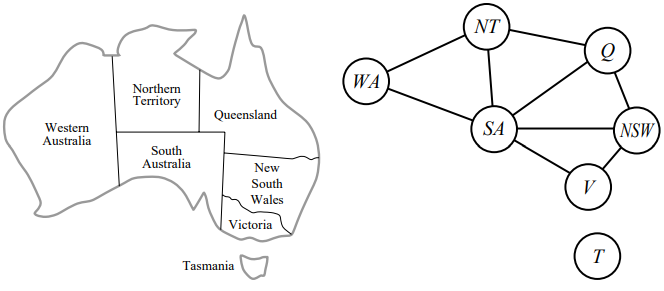
\includegraphics[width=15cm, keepaspectratio]{img/map_colouring.png}
	\caption{Map-colouring}\label{fig:map_colouring}
\end{figure}
\begin{figure}[H]
	\centering
    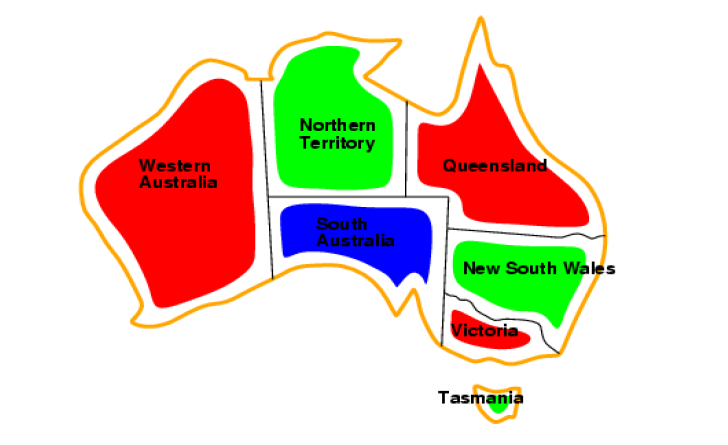
\includegraphics[width=14cm, keepaspectratio]{img/sol_map_coulouring.png}
	\caption{Soluzione Map-colouring}\label{fig:sol_map_colouring}
\end{figure}
In un CSP binario ogni vincolo è in relazione con due variabile. Il tipo più semplice di CSP coinvolge variabili che sono discrete e hanno domini finiti, i problemi di colorazione della mappa sono di questo tipo.
\paragraph{Tipi di variabili.} Le variabili discrete possono avere domini:
\begin{itemize}
    \item \textbf{finiti}: grandezza dell'assegnamento completo $d \longrightarrow O(d^n)$;
    \item \textbf{infiniti}: \begin{itemize}
        \item hanno bisogno di un linguaggio di vincoli
        \item i vincoli lineari sono risolvibili, i non lineari sono indecidibili;
    \end{itemize}
\end{itemize}
Le variabili continue con dei vincoli lineari sono risolvibili in un tempo polinomiale dai metodi LP. 

\paragraph{Tipi di vincoli.} I vincoli possono essere:
\begin{itemize}
    \item \textbf{unari}: coinvolgono una sola variabile;
    \item \textbf{binari}: coinvolgono due variabili;
    \item \textbf{higher-order}: coinvolgono 3 o più variabili;
    \item \textbf{preferenze}: es. \textit{il rosso è meglio del verde}, spesso rappresentabili come un costo associato a ogni assegnamento di variabile.
\end{itemize}
Inoltre i vincoli possono essere espressi in maniera:
\begin{itemize}
    \item \textbf{Implicita}: non viene direttamente indicata la relazione fra gli elementi del dominio che sono permessi. Un esempio può essere x<y, dove non si elencano tutti i possibili assegnamenti delle variabili che non violano quel vincolo ma si possono calcolare;
    \item \textbf{Esplicita}: si elencano tutti i valori ammessi per le variabili coinvolte nel vincolo. Nell'esempio di prima si avranno tutte le coppie di valori ammessi in base a quel vincolo.
\end{itemize}
\subsection{Caratteristiche CSP}
Alcune caratteristiche di questi problemi sono:
\begin{itemize}
    \item Caso speciale di un problema di ricerca;
    \item I domini possono essere discreti o continui;
    \item Commutatività: l'ordine in cui applichiamo le azioni non ha effetto: ad ogni nodo, considera solo le assegnazioni ad una singola variabile;
    \item Durante la ricerca, una volta violato un vincolo, rimane tale (monotonicità): fermati e torna indietro non appena un vincolo viene violato;
    \item L'ordine in cui scegliamo le variabili e i loro valori fa una grande differenza: abbiamo bisogno di un'euristica intelligente;
    \item Il test dell'obiettivo è scomposto in un insieme di vincoli sulle variabili, piuttosto che in una singola scatola nera;
    \item Quando gli insiemi di variabili sono indipendenti (nessun vincolo tra di loro) il problema è scomponibile in sottoproblemi che possono essere risolti indipendentemente;
    \item A ogni passaggio dobbiamo verificare la coerenza. Abbiamo bisogno di metodi di propagazione dei vincoli.
\end{itemize}

\subsection{Standard search formulation }
Gli stati sono definiti dal valore assegnato finora:
\begin{itemize}
    \item \textbf{Stato iniziale}: assegnamento vuoto \{\};
    \item \textbf{Funzione successore}: assegna un valore a una variabile non assegnata che non va in conflitto con l'assegnamento corrente;
    \item \textbf{Goal test}: l'assegnamento corrente è completo.
\end{itemize}
Questa formula viene usata per tutti i CSP e ogni soluzione appare a profondità n con n variabili. Il cammino è irrilevante, così che può usare la formulazione complete-state.


\section{Metodi di ricerca sistematici}
\subsection{Generate \& test}
Probabilmente il metodo di risoluzione dei problemi più generale. L'algoritmo consiste nei seguenti due passaggi che si ripetono:
\begin{enumerate}
    \item si generano le etichette;
    \item si controlla se vanno bene gli assegnamenti.
\end{enumerate}
Alcuni possibili miglioramenti sono ad esempio uno \textbf{smart generator}, ovvero si assegnano i valori alle variabili e se non vanno bene si effettuano dei cambiamenti sugli assegnamenti errati (ricerca locale). Un altro miglioramento consiste nel fare il test sugli assegnamenti e poi fare backtracking. 
\subsection{Backtraking}
Supponiamo di avere un problema CSP con 4 variabili (A,B,C,D), supponiamo che i vincoli siano 
\[A=D, B \neq D, A+C < 4\]
L'algoritmo consiste in:
\begin{enumerate}
    \item assegna il valore alla variabile;
    \item si controlla la consistenza;
    \item ripeti 1 e 2 finché tutte le variabili sono etichettate.
\end{enumerate}

\begin{figure}[H]
	\centering
    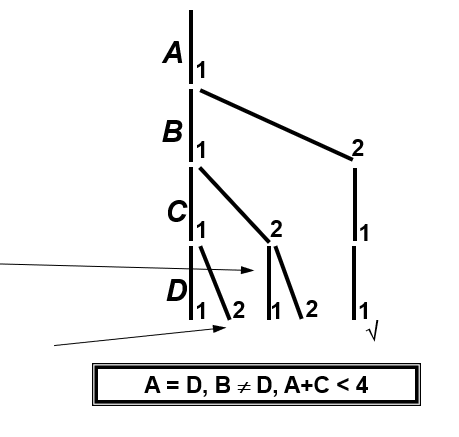
\includegraphics[width=7cm, keepaspectratio]{img/backtrack.png}
	\caption{Esempio backtracking.}\label{fig:es_backtracking}
\end{figure}
\noindent Se tutte le variabili non sono etichettate si torna al passo 1. 
 L'assegnamento delle variabili è commutativo ad esempio 
\begin{center}
  [WA = red allora NT = green] come [NT=green allora WA =red]  
\end{center}

\noindent Si devono solo considerare gli assegnamenti alle singole variabili per ogni nodo $\longrightarrow b = d $ e ci sono $d^n$ foglie.
La \textbf{DFS} per i CSP son gli assegnamenti a variabili singole è chiamata ricerca \textbf{backtracking}, essa è l'algoritmo base uniformed per i CSP.

\begin{figure}[H]
	\centering
    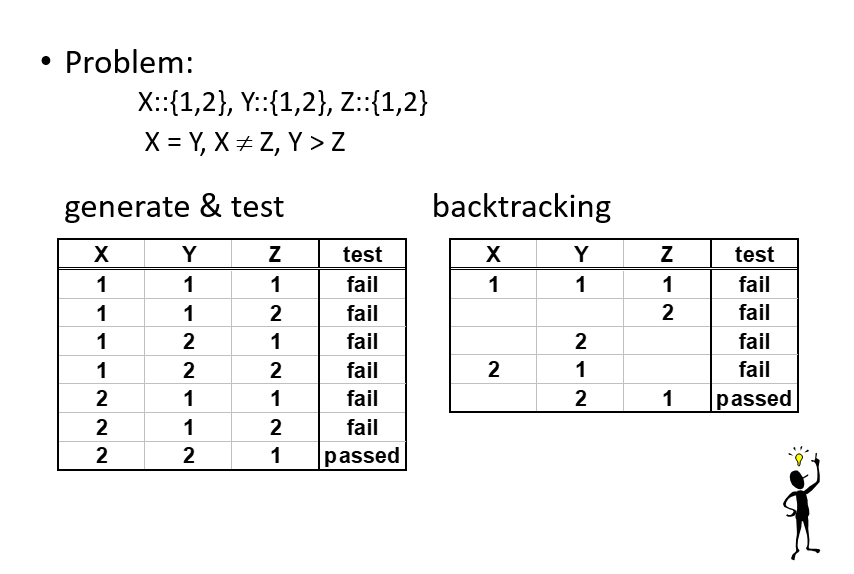
\includegraphics[width=13.5cm, keepaspectratio]{img/diff_generate_backtracking.png}
	\caption{Esempio generate and test vs backtracking.}\label{fig:diff_generate_backtracking}
\end{figure}

\subsubsection{Ricerca backtracking: incrementale}
La strategia di ricerca è la\textbf{ DFS (Depth First Search):}
\begin{enumerate}
    \item scegli una variabile non istanziata, scegli un valore dal suo dominio, controlla se qualche vincolo è violato;
    \item se nessun vincolo viene violato, continua la ricerca in modo ricorsivo;
    \item altrimenti, torna indietro: torna alla decisione precedente e fai un'altra scelta.
\end{enumerate}
In termini di grandezza dell'albero di ricerca il numero di foglie è pari a $d^n$, dove n è il numero di variabili e d = $max|D_i|$.
\begin{figure}[H]
	\centering
    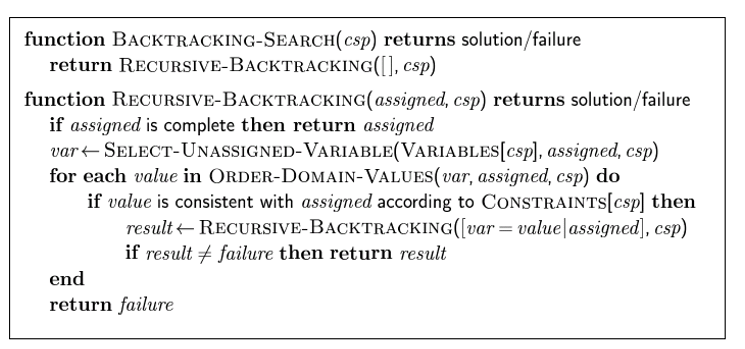
\includegraphics[width=14cm, keepaspectratio]{img/alg_backtracking.png}
	\caption{Algoritmo di backtracking.}\label{fig:alg_backtracking}
\end{figure}

\begin{figure}[H]
	\centering
    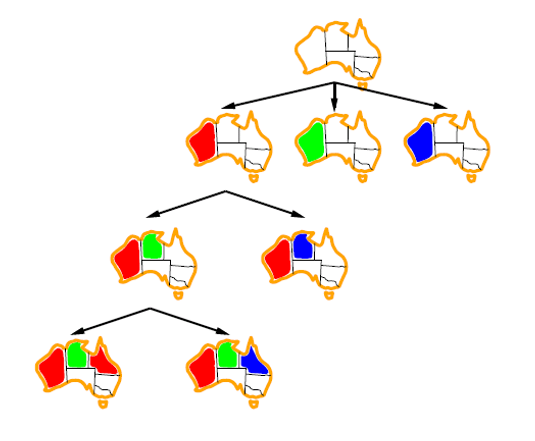
\includegraphics[width=10cm, keepaspectratio]{img/es_backtracking.png}
	\caption{Esempio backtracking.}\label{fig:es_backtracking}
\end{figure}

\subsection{Miglioramenti dell'efficienza del backtracking}
Per impostazione predefinita, SELECT-UNASSIGNED-VARIABLE seleziona semplicemente la successiva variabile non assegnata nell'ordine dato dalla lista VARIABLES[csp]. Questo ordinamento di variabili statiche raramente si traduce nella ricerca più efficiente. Ad esempio, dopo le assegnazioni per WA = rosso e NT = verde, c'è un solo valore possibile per SA, quindi ha senso assegnare SA = blue dopo piuttosto che assegnare Q. Infatti, dopo l'assegnazione di SA, le scelte per Q, NSW e V sono tutte forzate.
\paragraph{Variabile più vincolata} In questo caso si va a scegliere fra le variabili disponibili per l'assegnamento quella più vincolata in base ad alcune caratteristiche:
\begin{itemize}
    \item si sceglie la variabile con il \textbf{minor numero di valori legali} (minimum remaining values -MRV). È stata anche chiamata la "variabile più vincolata" o euristica "fail-first", quest'ultima perché seleziona una variabile che ha maggiori probabilità di causare un errore presto, potando così l'albero di ricerca.
    \begin{figure}[H]
    	\centering
        
\includegraphics[width=12cm, keepaspectratio]{img/impr_fewest_legal_values.png}
        \label{fig:fewest_legal_values}
    \end{figure}
    \item si sceglie la variabile con \textbf{più vincoli possibili} (degree heuristic) sulle variabili rimanenti.
    \begin{figure}[H]
    	\centering
        
\includegraphics[width=12cm, keepaspectratio]{img/most_constraints.png}
        \label{fig:most_costraint}
    \end{figure}
    \item data una variabile, si sceglie \textbf{il valore meno vincolante} (least-constraining-value), quello che esclude il minor numero di valori nelle restanti variabili.
    \begin{figure}[H]
    	\centering
        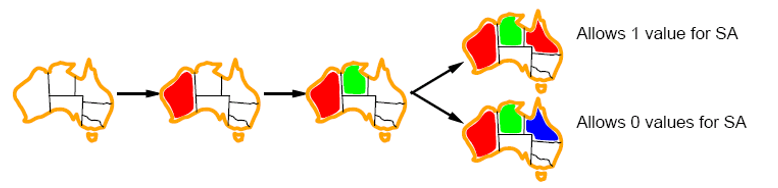
\includegraphics[width=13cm, keepaspectratio]{img/least_constraining_value.png}
        \label{fig:least_constraining_value}
    \end{figure}
\end{itemize}

\section{Propagazione delle informazioni attraverso vincoli}
Finora il nostro algoritmo di ricerca considera i vincoli su una variabile solo nel momento in cui il variabile viene scelta da SELECT-UNASSIGNED-VARIABLE. Ma guardando alcuni dei
vincoli all'inizio della ricerca, o anche prima dell'inizio della ricerca, possiamo drasticamente ridurre lo spazio di ricerca.

\subsection{Forward Checking}

Un modo per fare un uso migliore dei vincoli durante la ricerca è chiamato \textbf{forward checking}(controllo in avanti). Ogni volta che viene assegnata una variabile X, il processo di forward checking esamina ogni variabile non assegnata Y che è connessa a X da un vincolo e cancella dal dominio di Y qualsiasi valore non coerente con il valore scelto per X.
\begin{figure}[H]
    \centering
    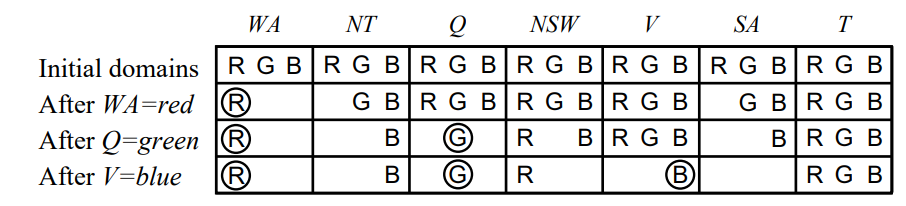
\includegraphics[width=13cm, keepaspectratio]{img/forward_checking.png}
    \caption{Forward checking applicata a Map-colouring problem.}\label{fig:forward_checking}
\end{figure}

Ci sono due punti importanti da notare su questo esempio. Innanzitutto, si noti che dopo aver assegnato WA = rosso e Q = verde, i domini di NT e SA
sono ridotti ad un unico valore; abbiamo eliminato del tutto la ramificazione su queste variabili grazie alla propagazione delle informazioni da WA e Q. L'euristica MRV, che è un partner ovvio per il controllo in avanti, selezionerebbe automaticamente SA e NT successivamente.

\subsection{Constraint propagation}
Sebbene il forward checking rilevi molte incoerenze, non le rileva tutte. Per esempio, consideriamo la terza riga della Figura \ref{fig:forward_checking}. Essa mostra che quando WA è rosso e Q è verde, sia NT che SA sono costretti a essere blu ma questo non è possibile perchè sono due zone vicine. Il forward checking non rileva questo come un'incoerenza, perché non guarda abbastanza avanti. La propagazione del vincolo (constraint propagation) è il termine generale per propagare le implicazioni di un vincolo su una variabile su altre variabili; in questo caso dobbiamo propagare da WA e Q su NT e SA, e quindi sul vincolo tra NT e SA per rilevare l'incoerenza. 

\subsubsection{Domain Consistency} L'idea di \textbf{arc consistency} fornisce un metodo veloce di propagazione dei vincoli sostanzialmente più forte del forward checking.
Una variabile è \textbf{consistente al dominio} (domain consistent) se nessun valore del dominio del nodo è è dichiarato impossibile da uno qualsiasi dei vincoli. L'idea è di "potare" il più possibile prima di selezionare un valore per le variabili. La domain consistency è stata definita solo per i vincoli che coinvolgono una sola variabile. Quando i vincoli sono binari, possiamo usare gli archi per indicare che un vincolo vale tra una coppia di variabili:
\begin{itemize}
    \item un \textbf{nodo} per ogni variabile;
    \item un \textbf{arco} per ogni vincolo.
\end{itemize}

\paragraph{Node Consistency.} In questo caso tutti i vincoli sono unari, le variabili sono rappresentate da dei \textbf{vertici}. Il vertice è \textbf{node consistent} se ogni valore nel dominio delle variabili soddisfa tutti i vincoli unari imposti sulla variabile X. Spesso vengono rappresentati come un cappio o arco che ritorna sullo stesso nodo. 
\begin{figure}[H]
    \centering
    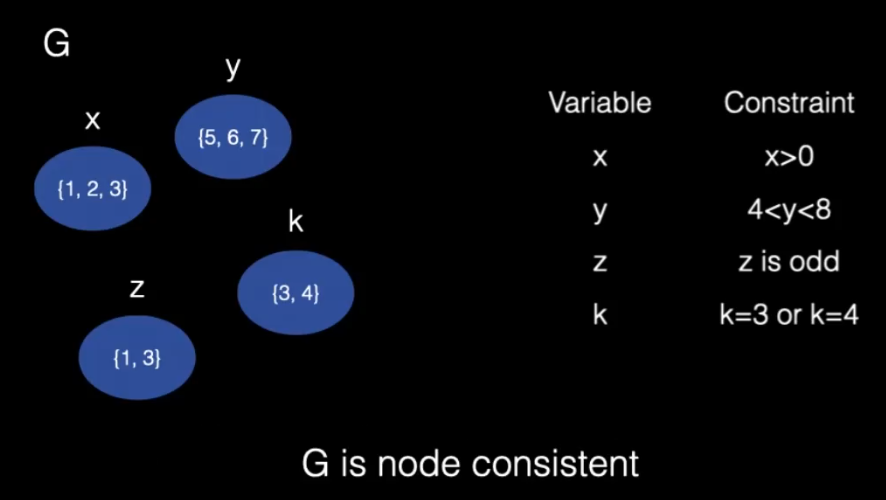
\includegraphics[width=13cm, keepaspectratio]{img/node_consistency.png}
    \caption{Esempio grafo node consistent.}\label{fig:node_consistency}
\end{figure}

\paragraph{Arc Consistency.} 
Quando tutti i vincoli sono binari si parla di \textbf{arc consistency}. Un arco (u,c) è consistente se per ogni valore x del dominio dom(u) esiste un valore y nel dom(v) tale che un assegnamento u=x e v=y soddisfa tutti i vincoli binari che coinvolgono sia u che v.

\subparagraph{Arc Consistency Algorihtm.} Per fare diventare un arco (u,v) consistente si cancellano tutti i valori x dal dom(u) che sono incosistenti con tutti i valori in dom(v). Restituisce true se è stata fatta una modifica al dominio di u.
\begin{figure}[H]
    \centering
    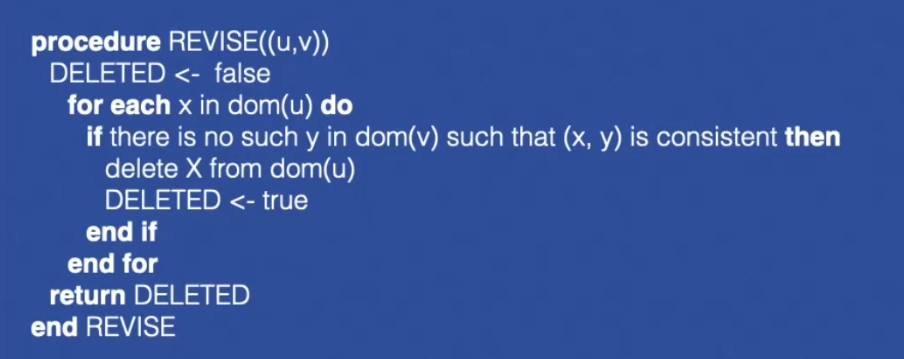
\includegraphics[width=13cm, keepaspectratio]{img/arc_consistency.png}
    \caption{Procedura REVISE.}\label{fig:arc_consistency}
\end{figure}


\subparagraph{AC-1} Un singolo passo dell'agoritmo REVISE non è sufficiente. L'algoritmo base per arc consistecy è AC-1, il quale esegue l'algoritmo REVISE finchè il dominio delle variabili cambia. In questo si ripete la procedura REVISE ogni volta che viene modificato un valore in un dominio.
\begin{figure}[H]
    \centering
    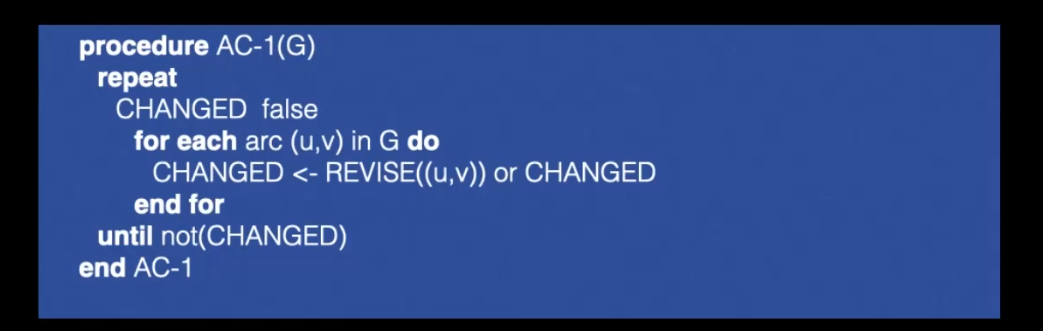
\includegraphics[width=13cm, keepaspectratio]{img/ac1_real.png}
    \caption{Algoritmo AC-1.}\label{fig:ac1}
\end{figure}
Una sola revisione riuscita di un arco su una particolare iterazione causa la revisione di tutti gli archi nella prossima iterazione anche se gli archi non sono influenzati dal cambiamento.

\subparagraph{AC-2}
AC-2 è un algoritmo che può fare arc consistecy in un solo passo attraverso i nodi. Il risultato è ottenuto passando per i nodi in un ordine numerico:
\begin{itemize}
    \item allegare ad un nodo tutti i valori che non sono in conflitto con i nodi precedentemente assegnati;
    \item Guardando i vicini di questo nodo che sono stati già valutati; se un valore non ha un'assegnazione corrispondente per lo stesso arco, eliminalo;
    \item Ogni volta che qualsiasi valore è cancellato da un arco, guarda ai suoi vicini a sua volta, e si controlla se un loro valore può essere eliminato. Se può essere eliminato, si continua il processo iterativamente finchè non ci sono più cambiamenti che possono essere fatti. Poi si prosegue con gli altri archi.
\end{itemize}
In sostanza si sceglie un ordine fra i nodi, prendiamo ad esempio y come primo e controlliamo tutti i vincoli fra y e k se c'è qualche valore di dom(y) che va in conflitto allora si elimina. Stessa cosa si per l'arco (x,y) se si fa qualche modifica si rimette in coda l'arco in modo da controllare se ci sono altre modifiche da fare. Se un valore b del nodo i è rimosso allora si aggiunge tutti (k,i) alla coda Q, per il controllo degli archi.
\begin{figure}[H]
    \centering
    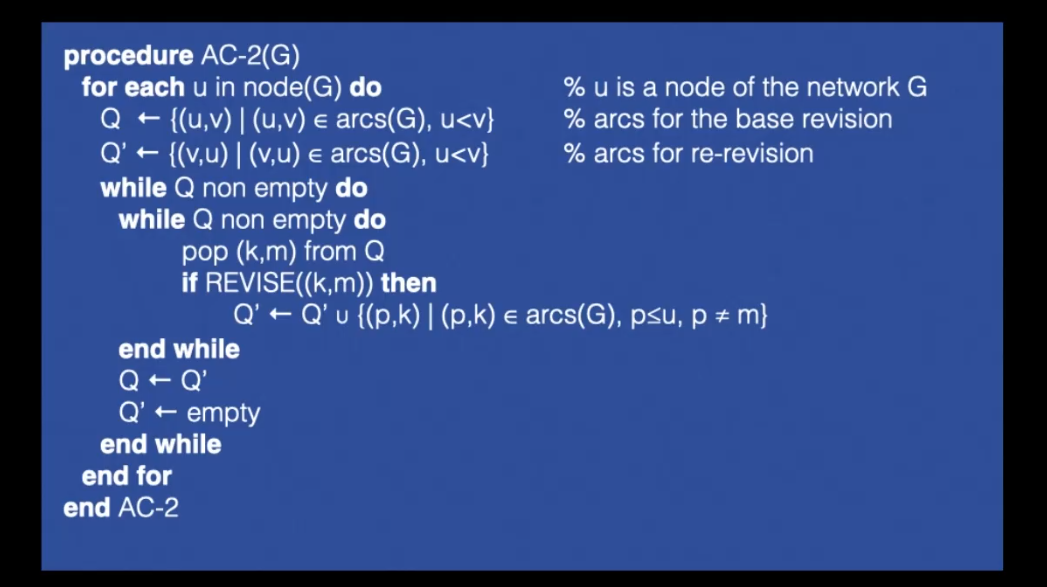
\includegraphics[width=13cm, keepaspectratio]{img/ac-2.png}
    \caption{Algoritmo AC-2.}\label{fig:ac2}
\end{figure}

\subparagraph{AC-3}
AC-3 è un miglioramento di AC-2, alcuni di essi possono essere già essere nella coda Q. Se è così allora non dovrebbero essere inseriti di nuovo. 
\begin{figure}[H]
    \centering
    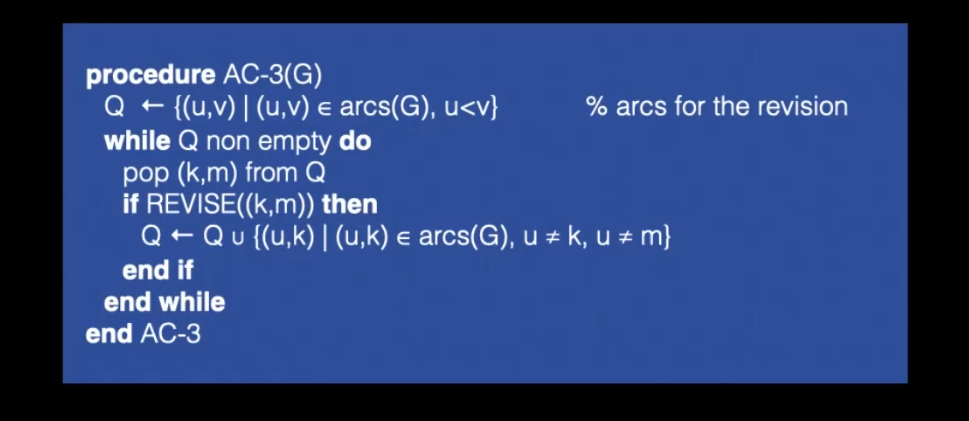
\includegraphics[width=13cm, keepaspectratio]{img/ac3.png}
    \caption{Algoritmo AC-3.}\label{fig:ac3}
\end{figure}
In sostanza si prende un arco dalla coda Q, si fa la REVISE, se faccio una modifica allora si aggiunge alla coda Q tutti gli archi (u,k) che non sono stati già controllati ovvero $u \neq k$ e $u\neq m$.
\section{Soft Constraint Satisfaction Problems}
I vincoli che abbiamo visto in precedenza sono dei vincoli \textbf{assoluti}, la cui violazione esclude una possibile soluzione. Molti dei problemi CSP reali includono i vincoli \textbf{preference} i quali indicano quali soluzioni sono preferite. Per esempio in un problema di timetable in università ci potrebbe essere il professore X che preferisce insegnare la mattina mentre il professore Y preferisce insegnare il pomeriggio. Un timetable dove il prof X insegna alle 14 e il prof Y alle 9 potrebbe essere una soluzione, ma non è quella ottimale viste le preferenze. I vincoli sulle preferenze possono essere codificati spesso come dei \textbf{costi} applicati sugli assegnamenti individuali delle variabili. Riprendendo l'esempio di prima possiamo dare all'assegnamento prof X = (lezione alle 14) un costo di 2, mentre all'assegnamento prof X = (lezione alle 9) un costo di 1. In questo modo si cerca fra le possibili soluzioni quella ottimale andando a minimizzare (o massimizzare...) il costo della soluzione. \\
Supponiamo di avere un problema di colorazione del grafo e cerchiamo di trovare una soluzione ottimale. 
\begin{figure}[H]
    \centering
    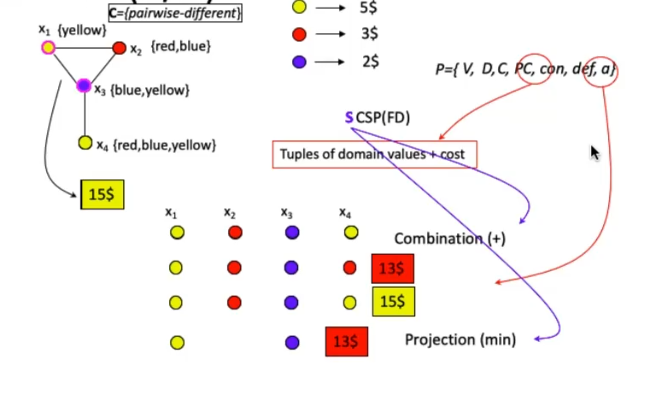
\includegraphics[width=12cm, keepaspectratio]{img/scsp_grafo.png}
    \caption{Esempio di SCSP su grafo.}\label{fig:scps_grafo}
\end{figure}

Partiamo riprendendo la definizione di un CSP, esso è definito come P=\{V,D,C,PC,con,def,a\} i quali indicano:
\begin{itemize}
    \item V= insieme delle variabili;
    \item D= insieme dei domini associati alle variabili;
    \item C= insieme di vincoli, definito come l'associazione variabile-vincolo ovvero quali variabili sono coinvolte in quale vincolo;
    \item PC= sono i vincoli primitivi e variano in base al vincolo e al dominio. A seconda del tipo di vincolo che possiamo avere i primitivi possono essere diversi, esempio se lavoro sugli interi esso conterrà vincoli con gli operatori <,>,= . Sostanzialmente esso indica i tipi di vincoli che posso usare se lavoro su un dominio specifico. Inoltre indicano se il vincolo è implicito (tutti i colori diversi) o esplicito (valgono le coppie <r,g,b>, <g,r,b>, …).
    \item con= funzione che definisce quali variabili sono coinvolte in quale vincolo, essa dato un vincolo restituisce le variabili che sono connesse a questo;
    \item def= funzione che indica quali sono i valori del dominio possibili per una specifica variabile. In un SCSP questa funzione oltre a dire i valori possibili per una variabile deve indicare anche il costo associato a quei valori, nell'esempio in Figura \ref{fig:scps_grafo} se passiamo in input alla funzione def la variabile $x_1$ essa ci ritornerà come valori possibile il colore giallo con costo 5\$. Questa è la differenza con la funzione def di un problema CSP.
    \item a= sottoinsieme di V contenente tutte le variabili interessate nella soluzione del SCSP, ad esempio nel caso del grafo abbiamo che le variabili che ci interessano per la soluzione ottimale sono solo $x_1$ e $x_3$, non tutte quante.
\end{itemize}
Nell'esempio in Figura \ref{fig:scps_grafo} i vincoli binari sono hard, perché la soluzione richiede per forza che i nodi collegati abbiamo colori diversi sennò si violano i vincoli, mentre i vincoli unari (quelli del costo sul colore) sono soft.
Nel caso di un CSP quando utilizziamo un algoritmo di ricerca per trovare una soluzione esso si può fermare alla prima soluzione che trova oppure, se richiesto, le cerca tutte quante. Nel caso di SCSP siamo costretti a trovare tutte le possibili soluzioni in modo da scegliere la migliore.
Normalmente si utilizzano due operazioni per trovare la soluzione ottimale in un SCSP:
\begin{itemize}
    \item \textbf{Combinazione (+)}: dove metto insieme tutti gli assegnamenti, combinando i vincoli, quindi si calcola anche il costo totale ad esempio con l'operazione di somma;
    \item \textbf{Proiezione ($\times$)}: operazione di scelta della soluzione migliore data dalla combinazione in base al minimo o al massimo del costo.
\end{itemize}
\subsection{Semiring}
Un semiring <A,+,$\times$,0,1> è una struttura costituita dai seguenti simboli:
\begin{itemize}
    \item \textbf{A}: l'insieme degli elementi che mi rappresentano i costi, quindi il dominio dei costi, esso può essere l'insieme dei reali oppure un intervallo specifico [0,1]
    \item \textbf{+}: operatore di proiezione, usato per fare la scelta fra le soluzioni trovate dalla combinazione, può essere il minimo o massimo. Possiamo definire alcune proprietà:
    \begin{itemize}
        \item \textbf{idempotente}: se faccio a+a dove l'operatore + è il minimo il risultato è sempre a, quando un operatore è idempotente è possibile definire un ordinamento ovvero 
        \[ a \leq b \text{ b è meglio di a } \iff a+b=b\]
    \end{itemize}
    \item \textbf{$\times$}: operatore di combinazione, utilizzato per combinare i vincoli, può essere somma,moltiplicazione etc... dipende dal problema. Possiamo definire alcune proprietà:
    \begin{itemize}
        \item \textbf{commutativa}: si considera il set di vincoli invece delle tuple.
    \end{itemize}
    \item \textbf{0}: rappresenta il valore minimo (peggiore) dell'insieme A, ovvero il bottom sotto il quale non si può andare, per l'intervallo [0,1] è 0;
    \item \textbf{1}: rappresenta il valore massimo (migliore) di A, il top, per l'intervallo [0,1] è 1. 
\end{itemize}
Tutti questi che abbiamo visto sono simboli quindi quando si utilizza l'operatore + non si ci si riferisce alla somma ma a un operatore per la proiezione che potrebbe essere minimo o massimo o or.

\subsubsection{Differenti tipi di semiring}
Esistono diversi tipi di semiring:
\begin{itemize}
    \item \textbf{Probabilistico}: <$\Re^+$, min, +, $+\infty$, 0> si minimizza la probabilità;
    \item \textbf{Weighted}: <[0,1],max,x,0,1> massimo il costo dato dalla combinazione, dove si fa il prodotto;
    \item \textbf{Fuzzy}: <[0,1],max,min,0,1>;
    \item \textbf{Classical}: <\{false,true\}, $\vee$, $ \wedge$, false, true>
\end{itemize}

\subsection{Local consistency}
Cerchiamo ora di vedere se è possibile applicare una tecnica di constraint propagation come arc consistency ai problemi SCSP in modo da rendere più efficiente la ricerca della soluzione. 
\subparagraph{Teorema dell'estensività} Se tolgo dei vincoli da un problema SCSP, la soluzione migliora perchè si moltiplica di meno (meno calcoli da fare),se li aggiungo la soluzione peggiora. Togliere vincoli vuol dire \textbf{rilassare} il problema.
\\
Se l'operatore x è idempotente allora possiamo applicare arc consistency, un esempio di operatore idempotente è il minimo se facciamo
\[1\times1= 2 \text{ dove $\times$ = somma}\]
\[1\times1= 1 \text{ se $\times$ = minimo}\]
Nei Semiring Fuzzy è possibile applicare arc consistency perchè $\times$ = min. Vediamo un esempio. 
\begin{figure}[H]
    \centering
    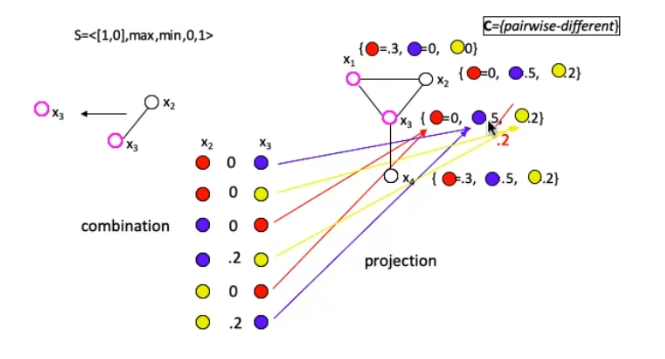
\includegraphics[width=12cm, keepaspectratio]{img/SCSP_arc_consistency.png}
    \caption{SCSP arc-consistency.}\label{fig:SCSP_arc_consistency}
\end{figure}
Nel caso dei SCSP quando si fa arc-consistency non si va a togliere elementi dal dominio ma si vanno a modificare i costi associati a quell'assegnamento. Ad esempio per il vincolo ($x_3$, $x_2$) andiamo a combinare tutti i vincoli e riportiamo tutte le coppie con i relativi costi, in questo caso si prende il minimo fra i due valori. E poi si proietta su $x_3$ i valori che abbiamo trovato e andiamo a modificare i costi associati ai colori, per $x_3$ = rosso e $x_3$ = giallo non cambiano perchè il $max_{rosso}(0,0) = 0$ e $max_{giallo}(0,0.2) = 0.2$ mentre per il blu abbiamo $max_{blue}(0,0.2) = 0.2$ quindi $x_3= 0.5 \xrightarrow{}0.2$.
\\
DA COMPLETARE 
\\
\chapter{Argumentation Framework}
\paragraph{Argumentation Framework.}Un argumentation framework (AF) è una coppia (A,R) dove 
\begin{itemize}
    \item A è un set di argomentazioni 
    \item $R \subseteq  A\times  A$ è una relazione rappresentante gli "attacchi" ("sconfitte")
\end{itemize}

\begin{center}
    F(\{a,b,c,d,e\}, \{(a,b),(c,b),(c,d),(d,c),(d,e),(e,e)\})
\end{center}
\begin{figure}[H]
    \centering
    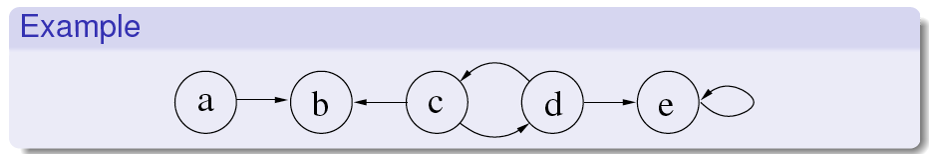
\includegraphics[width=12cm, keepaspectratio]{img/arg_fram.png}
    \caption{Argumentation framework.}\label{fig:arg_fram}
\end{figure}
Si ha un attacco quando si ha un'espressione logica (frase, dato...) che è in contraddizione con un'altra. Gli attacchi possono essere anche pesati, essi possono dipendere anche da chi ha detto quella frase.
\begin{figure}[H]
    \centering
    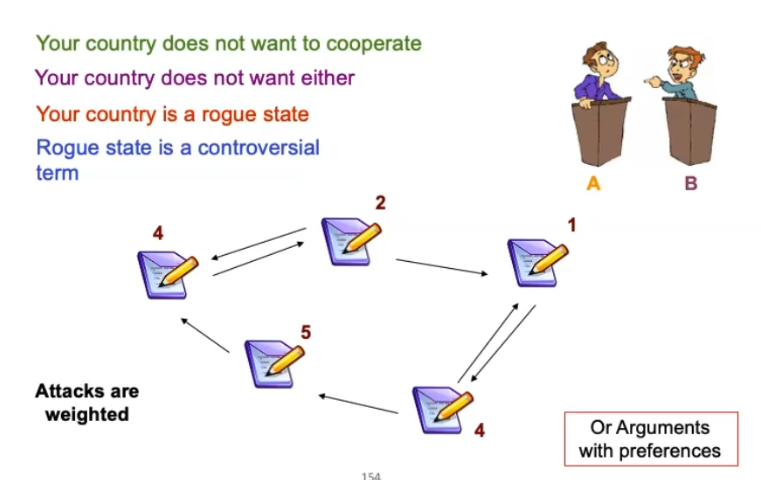
\includegraphics[width=12cm, keepaspectratio]{img/es_arg_fram.png}
    \caption{Esempio di argumentation framework.}\label{fig:es_arg_fram}
\end{figure}
Ci possono essere anche casi in cui è noto chi dice l'argomento e altri in cui non lo è. Per quest'ultima vogliamo selezionare gli argomenti che sono più validi rispetto agli altri, ad esempio in Figura \ref{fig:es_arg_fram} il 4 e il 2 sembrano buoni argomenti perchè attaccano gli altri e contrattaccano nel caso siano attaccati. Lo scopo è di definire dei criteri per trovare gli argomenti più forti, validi (che stanno "in piedi da soli"), in modo da selezione i conflitti che riescono a sopportare gli attacchi dall'esterno. 
\begin{figure}[H]
    \centering
    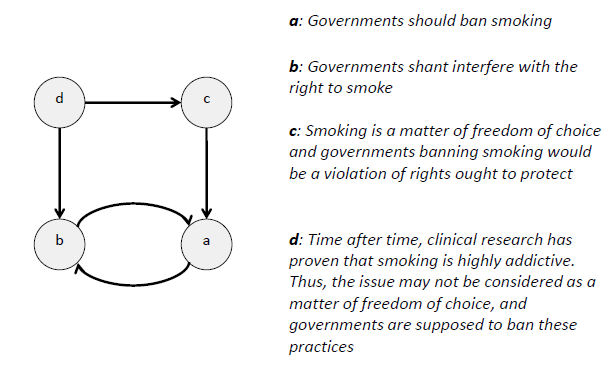
\includegraphics[width=13cm, keepaspectratio]{img/es_2_arg_fram.png}
    \caption{Altro esempio di argumentation framework.}\label{fig:es_2_arg_fram}
\end{figure}
Dobbiamo trovare gli argomenti che "stanno bene insieme", la prima nozione di questo tipo è un insieme di argomenti senza conflitti. 

\subsection{Extension-Based Semantics}
Queste solo le semantiche (criteri) che vanno a studiare i sottoinsiemi di argomenti per stabilire l'accettabilità degli stessi, ovvero se un argomento è un'estensione accettabile altrimenti viene rigettato.

\paragraph{Conflit-free extensions.} Dato un AF. F=(A,R). Un insieme $S\subseteq A$ è \textbf{conflict-free} in F, se, per ogni $a,b \in S ,(a,b) \notin R$.
\begin{figure}[H]
    \centering
    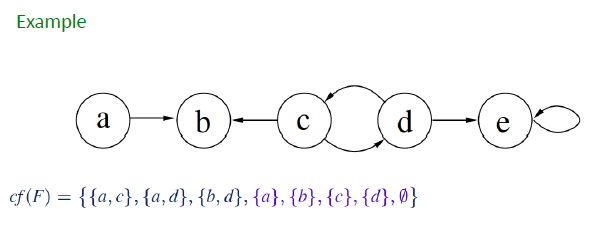
\includegraphics[width=13cm, keepaspectratio]{img/es_conflict_free.png}
    \caption{Esempio insieme conflict-free.}\label{fig:es_conflict_free}
\end{figure}
In questo caso andiamo a scegliere come coppie gli argomenti che non sono in conflitto (quindi che non si attaccano) fra di loro, (\{a,c\},\{a,d\} ma non \{a,b\}), e anche i singoli argomenti tranne e poichè esso si contraddice da solo visto che ha un cappio. 

\paragraph{Insiemi Ammissibili (Admissible).} Dato AF, F=(A,R). Un insieme $S \subseteq A$ è \textbf{ammissibile} in F, se 
\begin{itemize}
    \item S è conflict-free in F
    \item ogni $a\in S$ è difesa da S in F
    \begin{itemize}
        \item  $a\in A$ è difesa da S in F, se per ogni $b\in A$ con $(b,a) \in R$, esiste una $c\in S$, tale che $(c,b)\in R $
    \end{itemize}
\end{itemize}
Quindi gli insiemi admissible sono quelli senza conflitti e gli argomenti si difendono.
\begin{figure}[H]
    \centering
    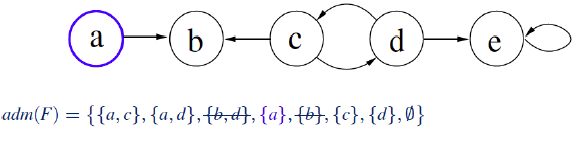
\includegraphics[width=13cm, keepaspectratio]{img/es_insieme_ammissibile.png}
    \caption{Esempio insieme ammissibile.}\label{fig:es_insieme_ammissibile}
\end{figure}
Non è necessario che sia lo stesso argomento a difendersi da altri attacchi, ad esempio in questo caso ,supponendo che non ci sia a, b è attaccato da c ma  se prendo d lui oltre che difendere se stesso da c (poichè attaccato) difende anche b. Guardando la definizione di difesa, un argomento a è difeso da un argomento b, $(b,a) \in R$, nel momento in cui esiste un argomento c tale che c attacca b, $(c,b) \in R$. Il sottoinsieme \{b,d\} non viene scelto poichè d è attaccato da c ma  si difende a sua volta contrattaccando, mentre b è attaccato sia da a che c, nel primo caso nessuno lo difende nel secondo d difende b perchè attacca c.

\paragraph{Insieme Completo (tutti difesi).} Dato un AF, F=(A,R). Un insieme $S \subseteq A$ è \textbf{completo} in F, se 
\begin{itemize}
    \item S è ammissibile in F
    \item ogni $a\in A$ difeso da S in F è contenuto in S
    \begin{itemize}
        \item $a\in A$ è difeso da S in F, se per ogni $b\in A$ con $(b,a) \in R$, esiste una $c\in S$, tale che $(c,b)\in R$.
    \end{itemize}
\end{itemize}
\begin{figure}[H]
    \centering
    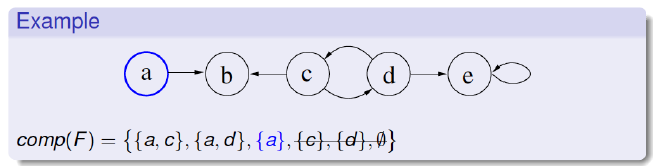
\includegraphics[width=13cm, keepaspectratio]{img/es_set_complete.png}
    \caption{Esempio insieme completo.}\label{fig:es_insieme_completo}
\end{figure}
Quindi un insieme complete contiene tutti gli insiemi ammissibili e anche tutti gli argomenti che sono difesi.

\paragraph{Grounded (scettica).} Dato un AF F=(A,R). Un insieme $S \subseteq A$ è \textbf{grounded} in F, se 
\begin{itemize}
    \item S è completo in F
    \item per ogni $T \subseteq A$ completo in $F,T \nsubseteq  S$.
\end{itemize}

\begin{figure}[H]
    \centering
    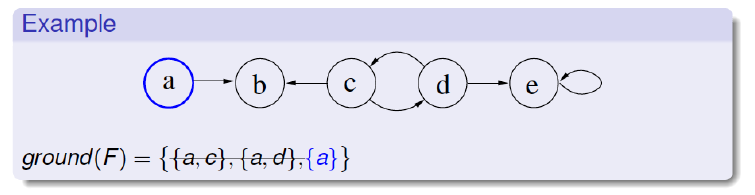
\includegraphics[width=13cm, keepaspectratio]{img/es_grounded.png}
    \caption{Esempio grounded.}\label{fig:es_insieme_grounded}
\end{figure}
Sceglie tra gli argomenti che sono nella complete, gli argomenti che compaiono in tutte le estensioni, è una semantica scettica perchè vuole essere sicuro che gli argomenti che sceglie provengano da una decisione prudente. 

\paragraph{Preferred.} Dato un AF, F= (A,R). Un insieme $S\subseteq A$ è \textbf{preferito} in F, se 
\begin{itemize}
    \item S è ammissibile in F
    \item per ogni $T\subseteq A$ ammissibile in T, $S\nsubseteq T$
\end{itemize}


\begin{figure}[H]
    \centering
    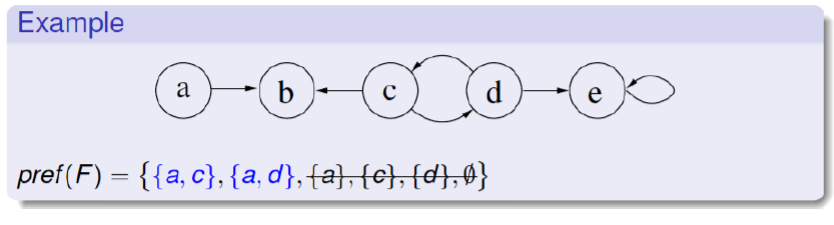
\includegraphics[width=13cm, keepaspectratio]{img/es_preferred.png}
    \caption{Esempio preferred.}\label{fig:es_insieme_preferred}
\end{figure}

Al contrario di grounded dove si andava a scegliere l'insieme con l'elemento in comune con gli altri insieme, in questo caso si va a scegliere tra gli insiemi ammissibili quelli che sono più grandi a livello di inclusione insiemistica. Da notare che si sceglie tra gli insiemi ammissibili ma si può dimostrare che si può scegliere da quelli complete.

\paragraph{Stable.} Dato un AF, F= (A,R). Un insieme $S\subseteq A$ è \textbf{stabile} in F, se
\begin{itemize}
    \item S è conflict-free in F
    \item per ogni $a\in A\setminus S$, esiste una $b\in S$, tale che $(b,a)\in R$. 
\end{itemize}

\begin{figure}[H]
    \centering
    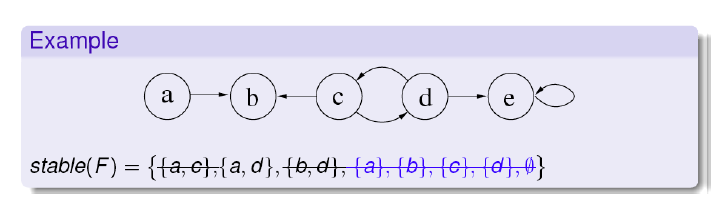
\includegraphics[width=13cm, keepaspectratio]{img/es_stable.png}
    \caption{Esempio insieme stable.}\label{fig:es_insieme_stable}
\end{figure}
In questo caso si sceglie l'insieme i quali elementi attaccano tutti gli elementi fuori dall'insieme conflict-free, ad esempio \{a,c\} non si prende perchè a attacca b e c attacca d e b ma nessuno dei due attacca e. Mentre nell'insieme \{a,d\} a attacca b e d attacca sia c che e. Esiste anche una semantica \textbf{semi-stabile} la quale nel caso cui esista un insieme stabile allora essa coincide con quest'ultimo ma quando non c'è la stabile allora sceglie tra gli insieme preffered quelli che ne attaccano di più tra gli insiemi fuori a quest'ultimo. L'obiettivo della semantica stabile è di avere  cardinalità più grande possibile e di attaccare tutti gli insiemi fuori.

\subsubsection{Complessità}
La complessità è descritta da due valori:
\begin{itemize}
    \item \textbf{Cred}: (credulous) rappresenta il costo associato all'operazione di controllo sulle semantiche, si controlla se un determinato insieme contiene un argomento passato;
    \item \textbf{Skept}: (scettico) controlla se un argomento è incluso in tutte le estensioni.
\end{itemize}

\subsection{Weighted AF}
Come abbiamo visto anche per i SCSP dove avevamo un costo applicato ai valori dei domini di una variabile, un weighted AF è costituito da archi pesati (attacchi pesati). Supponiamo di avere due argomentazione che si attaccano a vicenda:
\begin{itemize}
    \item A= la BBC dice che ci sarà il sole a Londra;
    \item B= la CNN dice che piove a Londra;
\end{itemize}
Queste due argomentazioni sono in contraddizione tra di loro ma non hanno lo stesso peso. Una possibile ragione per la quale  A è preferito a B è perchè la BBC è ritenuta più affidabile della CNN.
\subsubsection{Weighted Semirings WAAF}
Un AF basato sui semiring è una quadrupla $<A,R,W,S>$ dove 
\begin{itemize}
    \item S è un semiring <S,+,$\times$,$\perp $,$\top $>;
    \item A è un insieme di argomenti;
    \item R  l'insieme delle relazioni binarie, attacchi;
    \item W:A$\times$A$\xrightarrow{}S$ è una funzione binaria.
\end{itemize}
Dato a,b$\in$ A, $\forall(a,b)\in R$, W(a,b)=s vuol dire che a attacca b con un peso s$\in$S. Quello che andremo a studiare noi sono gli AF che hanno un peso assegnato all'arco e non al nodo.
\begin{figure}[H]
    \centering
    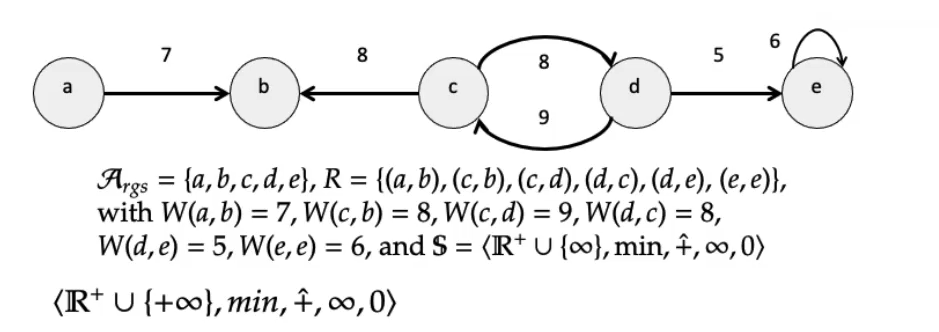
\includegraphics[width=14cm, keepaspectratio]{img/af_wighted.png}
    \caption{Esempio Af pesato.}\label{fig:es_AF_pesato}
\end{figure}

\subsubsection{W-defence $D_w$} 
Dato un WAAF, WF=$<A,R,W,S>$, B$\subseteq$ A w-difende b $\in$ A se e solo so, dato a$\in$ A e R(a,b), allora W(a, $B \cup \{b\} \geq_s W(B,a)$; B difende b se e solo difende b da qualsiasi a che lo attacca R(a,b).

\begin{figure}[H]
    \centering
    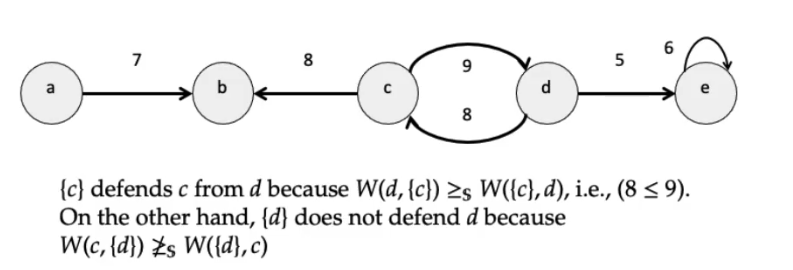
\includegraphics[width=14cm, keepaspectratio]{img/w_difesa.png}
    \caption{Esempio w-defence.}\label{fig:w_difesa}
\end{figure}
Dato un WAAF si dice che un insieme di argomenti è difeso se gli attacchi che partono da questo insieme verso degli attaccanti sono più forti (hanno un maggiore peso totale) rispetto agli attacchi ricevuti. Si parla di insieme di argomenti perché si va ad aggregare il peso degli attacchi. Ovvero supponendo che un argomento a attacca degli argomenti b e c con un peso di 2 e 3 rispettivamente, b e c possono coalizzarsi in modo da difendersi dall'attacco ricevuto singolarmente, l'insieme dei difensori deve coprire un peso che "mette insieme" il peso 2 e 3.   Questo vuol dire che bisogna scegliere un'operazione per il semiring in modo da calcolare chi vince tra gli attaccanti e i difensori. 
\paragraph{Martinez}
\begin{figure}[H]
    \centering
    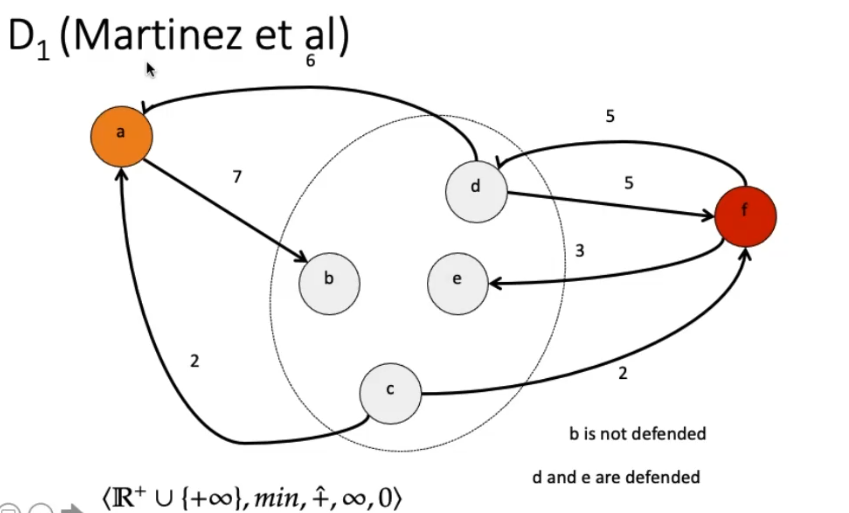
\includegraphics[width=14cm, keepaspectratio]{img/d1_martinez.png}
    \caption{Esempio approccio Martinez.}\label{fig:d1_martinez}
\end{figure}
In questo Esempio possiamo vedere che ci sono degli argomenti (c,b,e,d) che sono inseriti in un insieme (coalizione) in modo da difendersi dagli attacchi degli argomenti a e f. Vediamo che a attacca b con un attacco pari a 7, la coazione per difendersi da questo attacco deve rispondere con un attacco maggiore o uguale di questo. La coalizione attacca b con due attacchi di peso pari a 2 e 6 verso a, se avessimo fatto la somma dei pesi allora b sarebbe stato difeso ma in questo caso si va a prendere il \textbf{massimo} tra i due valori (semiring Martinez) ovvero 6. Ciò significa che b non è difeso dall'attacco di a perché la coalizione risponde con un attacco pari a 6<7.  Mentre d ed e sono difesi dall'attacco di f perché esso attacca con un valore massimo pari a 5 e la coalizione contrattacca con un valore sempre di 5. In questo tipo di approccio si va a prendere il massimo sia in attacco che in difesa.

\paragraph{Coste-Marquis}
\begin{figure}[H]
    \centering
    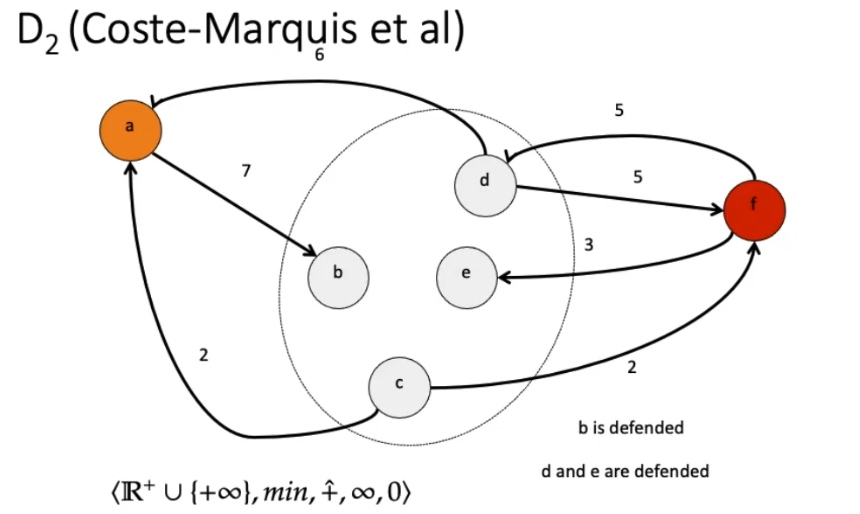
\includegraphics[width=14cm, keepaspectratio]{img/d2_coste_marquis.png}
    \caption{Esempio approccio Coste-Marquis.}\label{fig:coste_marquis}
\end{figure}
Con il metodo di Coste-Marquis si deve aggregare non l'attacco ma solo la difesa, infatti in questo caso b è difeso dalla coalizione perché risponde con un attacco pari a 6+2=8>7. Anche d ed e sono difesi perchè sono attaccati con un valore pari a 5 e rispondono con un attacco pari a 7. In sostanza si prende il massimo per l'attacco e si fa la somma in caso di difesa. 

\paragraph{Santini e Bistarelli}
\begin{figure}[H]
    \centering
    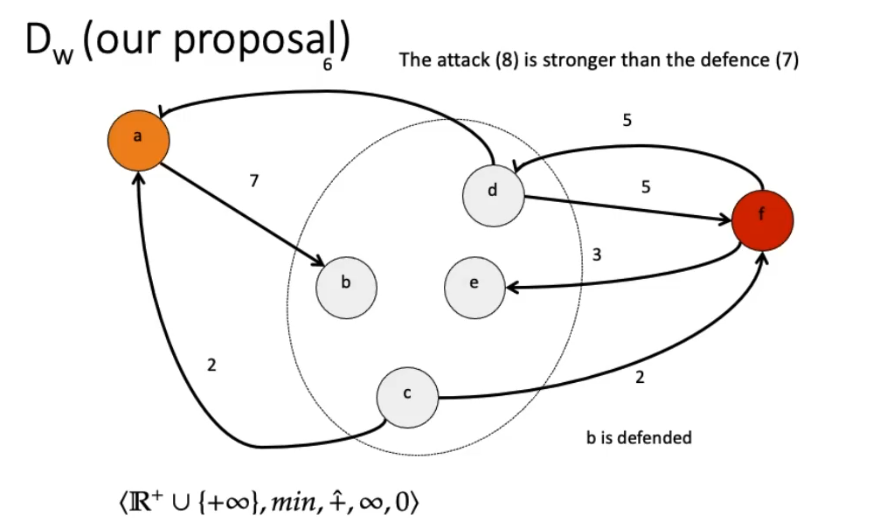
\includegraphics[width=14cm, keepaspectratio]{img/d_w_santini_bistarelli.png}
    \caption{Esempio approccio Santini e Bistarelli.}\label{fig:d_w_santini_bistarelli}
\end{figure}
Mentre nella proposta di Santini e Bistarelli si va ad aggregare sia l'attacco che la difesa, ciò vuol dire che b è difeso ma d ed e no. Quest'ultimi ricevono un attacco da parte di f pari a 5+3=8 e rispondo con un attacco pari a 5+2=7 che non è sufficiente per vincere.

\paragraph{Confronto risultati}
\begin{figure}[H]
    \centering
    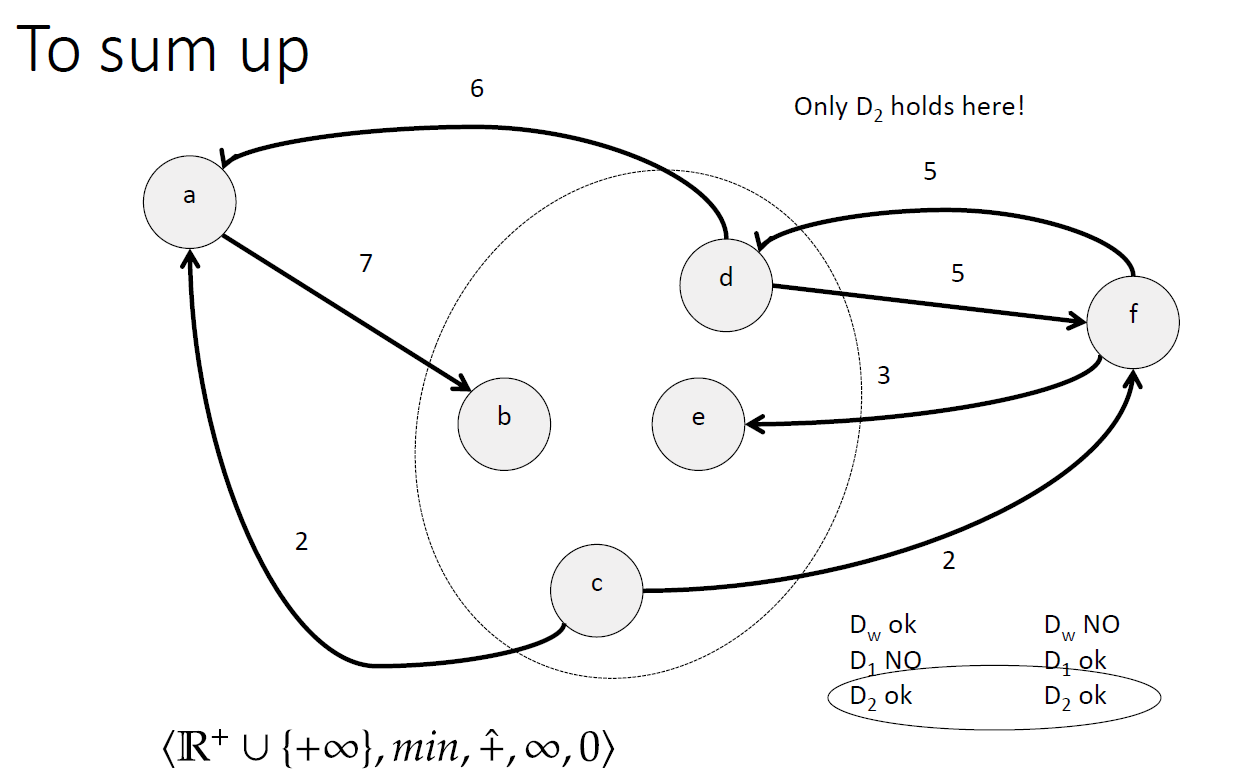
\includegraphics[width=13cm, keepaspectratio]{img/riassunto_d_waaf.png}
    \caption{Riassunto approcci D.}\label{fig:riassunto_d_waaf}
\end{figure}
Per riassumere un insieme è ammissibile se riesce a difendersi da tutti gli attacchi ricevuti, applicando i diversi metodi solo per Coste-Marquis questo insieme è ammissibile perchè la somma degli attacchi da parte della difesa verso un argomento attaccante è maggiore del valore massimo tra gli attacchi di quest'ultimo.

\paragraph{Semantiche in un WAAF}
Siccome la nozione di admissible è usata nella nozione di difesa dobbiamo adattare la semantica vista in precedenza a questo di framework. Essa terrà conto anche dei pesi applicati sugli archi, di seguito riporto la definizione di \textbf{w-conflict-free} ed \textbf{w-admissible}.
\begin{figure}[H]
    \centering
    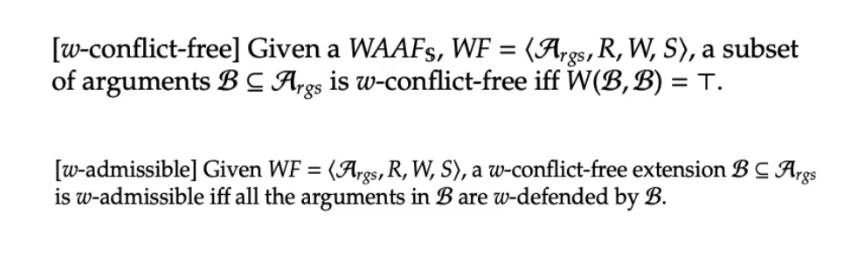
\includegraphics[width=14cm, keepaspectratio]{img/w_semantiche.png}
    \caption{Definizione semantiche in un WAAF.}\label{fig:w_semantiche}
\end{figure}

\paragraph{Esempio w-conflict-free ed admissible.}
Ansiamo ora a vedere un esempio delle semantiche applicate a un AF con i pesi. 
\begin{figure}[H]
    \centering
    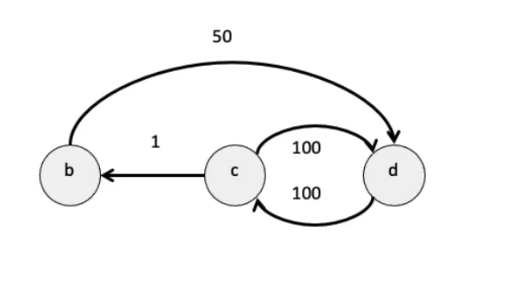
\includegraphics[width=11cm, keepaspectratio]{img/es_w_semantics.png}
    \caption{Esempio semantiche in WAAF.}\label{fig:es_w_semantics}
\end{figure}
Vediamo quale è l'insieme S conflict-free, sicuramente non (b,c), (c,d) e (b,d) visto che si attaccano:
\[S=\{ \emptyset,\{b\},\{c\},\{d\}\}\]
In questo caso si va a considerare anche il peso dell'attacco quindi l'insieme \{b,c\} è più w-conflict-free \{c,d\} perchè c attacca b con un peso di 1 mentre c e d si attaccano a vicenda con un peso di 100. Quindi b e c vanno più d'accordo rispetto a c e d, possiamo quindi decidere di mettere insieme b e c nonostante una leggera disputa interna in modo da avere una coalizione più forte in difesa contro gli attacchi dall'esterno. 
\subparagraph{Rilassamenti ortogonali.} Questi rilassamenti sono strettamente correlati e influenzano l'un l'altro: permettere un piccolo conflitto può portare ad avere più argomentazioni in un'estensione, e di conseguenza si ha una difesa più forte o più debole. Un esempio reale potrebbe essere in campo politico, partiti con piccole divergenze interne si uniscono in modo da raggiungere una percentuale sufficiente di voti per governare.


\subsection{Labelling-Based Semantics}
\subsubsection{Reinstatement Labelling}
Finora abbiamo visto delle estensioni in cui gli argomenti venivano accettati (validi, quelli che si trovavano all'interno delle estensioni) o rigettati. Con le labelling semantics manteniamo queste due sfumature e ne aggiungo un'altra ovvero gli argomenti vengono suddivisi in:
\begin{itemize}
    \item \textbf{IN}: argomenti accettati, sono IN se sono attaccati solo da argomenti OUT;
    \item \textbf{OUT}: argomenti rigettati, sono OUT se sono attaccati solo da argomenti IN;
    \item \textbf{UNDEC}: altrimenti, tutto il resto .
\end{itemize}
\begin{figure}[H]
    \centering
    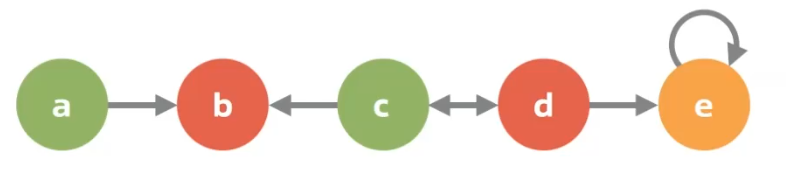
\includegraphics[width=13cm, keepaspectratio]{img/labelling_semantics_es.png}
    \caption{Esempio Reinstatement Labelling .}\label{fig:es_Reinstatement_Labelling}
\end{figure}

\paragraph{Conflict-free.}
Per ogni $a \in A$ si ha che:
\begin{itemize}
    \item se a è etichettata IN allora non ha un attaccante che è IN e
    \item se a è etichettata OUT allora ha almeno un attaccante che è IN
\end{itemize}
La Figura \ref{fig:es_Reinstatement_Labelling} è conflict-free perchè valgono le due regole citate per tutti gli argomenti. 

\begin{figure}[H]
    \centering
    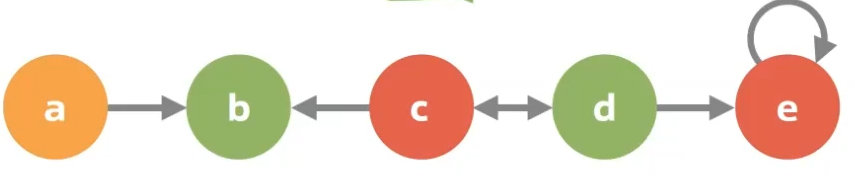
\includegraphics[width=13cm, keepaspectratio]{img/es_conflict_free_labelling.png}
    \caption{Esempio conflict-free con labelling .}\label{fig:es_conflict_free}
\end{figure}
Anche in questo caso abbiamo un insieme conflict-free.
\begin{figure}[H]
    \centering
    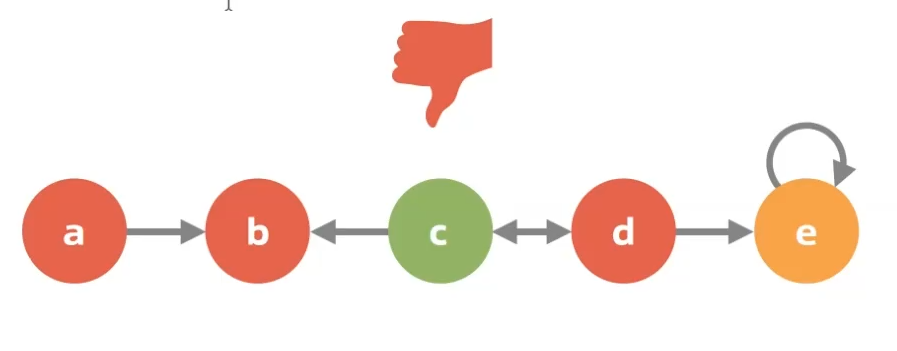
\includegraphics[width=13cm, keepaspectratio]{img/es_no_conflict_free_labelling.png}
    \caption{Esempio no conflict-free con labelling .}\label{fig:es_noconflict_free}
\end{figure}
In questo ultimo esempio non abbiamo un insieme conflict-free perchè a viene considerato OUT, quindi rigettato, anche se non viene attaccato da nessuno e infatti non ci sono attaccanti IN per quest'ultimo.

\paragraph{Admissible.}
Per ogni $a \in A$ si ha che:
\begin{itemize}
    \item se a è etichettata IN allora tutti gli attaccanti sono OUT e
    \item se a è etichettata OUT allora ha almeno un attaccante che è IN
\end{itemize}
L'interpretazione che possiamo dare alla prima regola è che un argomento IN è accettato come nell'insieme admissible se i suoi attaccati sono tutti sconfitti.
Riprendo l'esempio in Figura \ref{fig:es_Reinstatement_Labelling} è un insieme admissible, poichè a non è attaccato da nessuno quindi la prima condizione è vera e anche per c poichè essa è attaccata solo da argomenti OUT ovvero d. Anche l'esempio in Figura \ref{fig:es_conflict_free} è admissible.

\paragraph{Completo.}
Per ogni $a \in A$ si ha che:
\begin{itemize}
    \item a è etichettata IN \textbf{se e solo} se tutti gli attaccanti sono OUT e
    \item a è etichettata OUT\textbf{ se e solo se} ha almeno un attaccante che è IN
\end{itemize}
Quesro vuol dire che se un argomento è difeso deve stare per forza dentro l'estensione. Perciò un attaccante è IN se ha solo attaccanti OUT e viceversa se un argomento ha solo attaccanti OUT allora è per forza etichettato come IN. Stessa discorso vale per la seconda regola, dobbiamo vederla come divisa in due parti la parte di sinistra e di destra al se e solo. 

\begin{figure}[H]
    \centering
    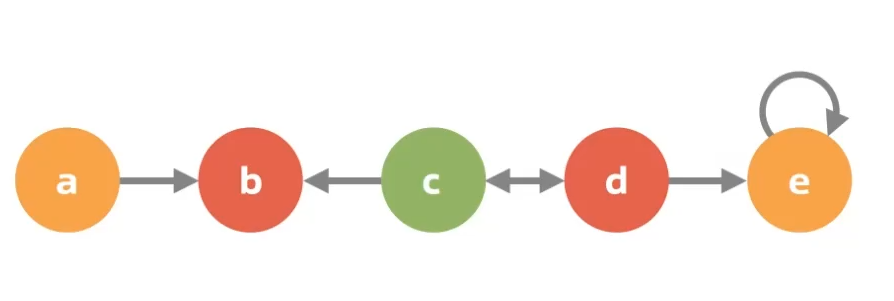
\includegraphics[width=13cm, keepaspectratio]{img/es_no_complete_labelling.png}
    \caption{Esempio no complete con labelling .}\label{fig:es_no_complete_labelling}
\end{figure}
In questo esempio non abbiamo un insieme complete perchè l'argomento a che è etichettato come UNDEC non ha attaccanti e quindi dovrebbe essere etichettato come IN.

\begin{figure}[H]
    \centering
    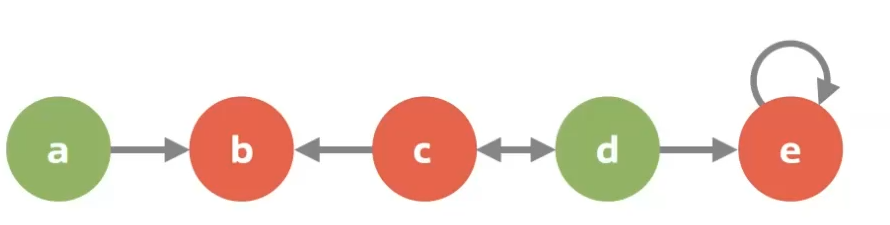
\includegraphics[width=13cm, keepaspectratio]{img/es_complete_labelling.png}
    \caption{Esempio  complete con labelling .}\label{fig:es_no_complete_labelling}
\end{figure}
Ogni etichettatura degli argomenti verifica le regole scritte in precedenza infatti a non ha attaccanti quindi è IN, b ha un attaccante IN quindi è OUT, c ha un attaccante IN quindi è OUT, d ha tutti attaccanti OUT ovvero c e per ultimo e potrebbe essere UNDEC ma essendo che ha almeno un attaccanti IN allora è considerato OUT.

\paragraph{Preferred.}
L'etichettatura
\begin{itemize}
    \item è un insieme complete, e 
    \item l'insieme di argomenti IN è \textbf{massimale} fra tutte le etichette complete.
\end{itemize}
In questo caso si ragiona sulla cardinalità quindi si va a prendere il numero maggiore di argomenti che sono considerati completi. Questa semantica è preferita nel caso in cui si vogliano tirare in ballo più argomenti e sentire più opinioni.

\paragraph{Grounded.}
L'etichettatura
\begin{itemize}
    \item è un insieme complete, e 
    \item l'insieme di argomenti IN è \textbf{minimale} fra tutte le etichette complete.
\end{itemize}
Invece per la grounded si vanno a prendere tutti i labelling complete e si sceglie quello in cui ho meno argomenti IN.

\begin{figure}[H]
    \centering
    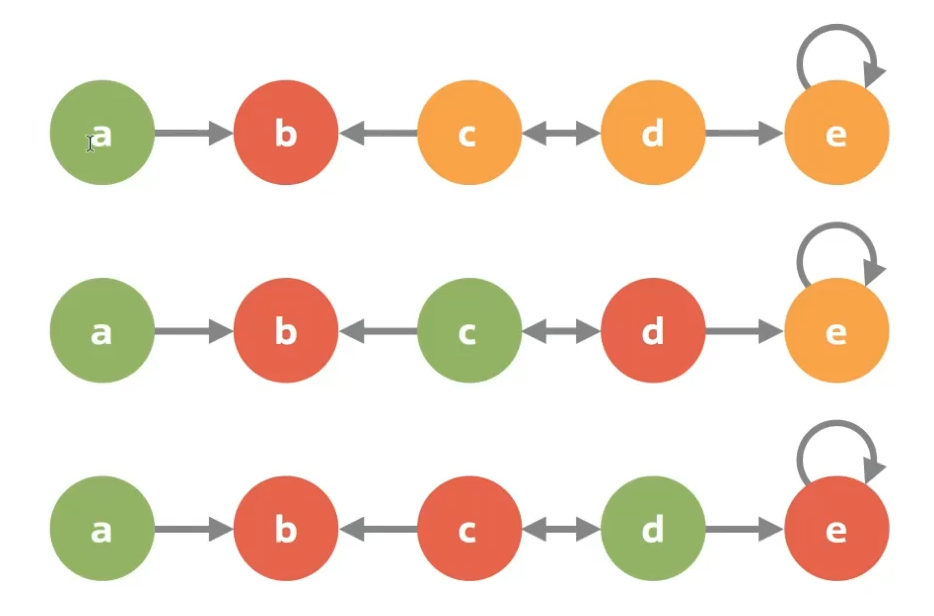
\includegraphics[width=13cm, keepaspectratio]{img/grounded_preferred.png}
    \caption{Esempi insiemi grounded e preferred .}\label{fig:es_grounded_preferred}
\end{figure}
Il primo è un esempio di insieme grounded, gli ultimi due sono preferred. Il secondo insieme è anche grounded perchè le etichette che sono state assegnate come IN sono minimali e massimali, supponiamo di mettere b e d a IN se b è IN non è complete perchè non ha attaccanti OUT stessa cosa vale per d se si etichetta come IN. Se invece assegniamo a c OUT l'insieme non è complete perchè c per essere OUT deve avere almeno un attaccante IN. Lo stesso discorso vale per l'ultimo esempio.
\subsection{Ranking-Based Semantics}
Si trasforma l'AF in un sistema di classificazione, in questo caso con le estensioni non si vanno a scegliere dei sottinsiemi di argomenti ma si a fare una classificazione di quest'ultimi. Per stabilire se un argomento è migliore di un altro si usano dei criteri per studiare la validità, ad esempio possono contare quanti attacchi diretti riceve un argomento o posso misurare la lunghezza dei path da un argomento a un altro etc... 

\paragraph{Categorizer.} Si tratta di una funzione di ranking degli argomenti, la quale assegna un valore agli argomenti controllando quali sono gli attaccanti diretti di questi.

\begin{figure}[H]
    \centering
    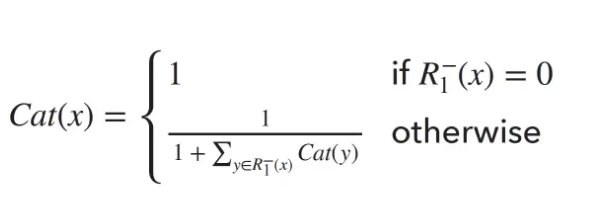
\includegraphics[width=13cm, keepaspectratio]{img/categorizer.png}
    \caption{Funzione categorizer .}\label{fig:fun_categorizer}
\end{figure}
Se un argomento non ha attaccanti $R^{-1}(x) = 0$ allora il valore è 1 sennò è dato dalla formula $\dfrac{1}{1+ \sum_{y \in R^{-1}(x)}^{}Cat(y)}$, questo significa che se ho attaccanti forti allora l'argomento x è debole.
\begin{figure}[H]
    \centering
    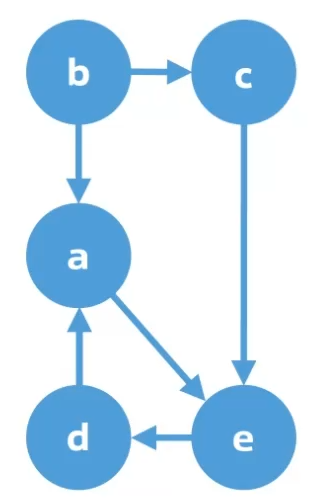
\includegraphics[width=5cm, keepaspectratio]{img/es_categorizer.png}
    \caption{Esempio categorizer .}\label{fig:es_categorizer}
\end{figure}
In questo caso Cat(b)=1 perchè non ha attaccanti e Cat(c)=0.5 perchè è attaccato da b con punteggio 1. Mentre Cat(a)=0.38, Cat(d) =0.65 e Cat(e) = 0.53 quindi la classificazione di questo insieme è 
\[b\succ^{Cat}d\succ^{Cat}e\succ^{Cat}c\succ^{Cat}a\]

\subsection{Graded semantics}
I principi sono simili a quello precedente:
\begin{itemize}
    \item più è grande il numero degli attaccanti su un argomento b, più è debole il livello di giustificazione di b
    \item più è grande il numero di argomenti che difendono a, più è forte il livello di giustificazione di a.
\end{itemize}

\subsubsection{Graded defense}
In questo caso andiamo a ricercare delle partizioni degli argomenti con $d_n^{m}(X)$, il quale è un insieme di argomenti che non hanno almeno m attaccanti che non sono contrattaccati da almeno n argomenti in X. Questo vuol dire che un argomento $a\in d_n^{m}(X)$ se non ci sono almeno m attaccanti che sono difesi da almeno n argomenti.
\begin{figure}[H]
    \centering
    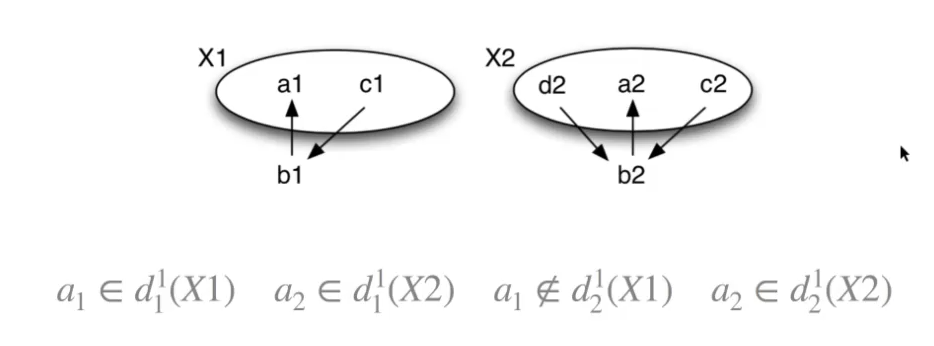
\includegraphics[width=13cm, keepaspectratio]{img/es_graded_defense.png}
    \caption{Esempio graded defense .}\label{fig:es_graded_defense}
\end{figure}

\paragraph{Ranking functions.} Le regole sono:
\begin{itemize}
    \item meno attaccanti ho meglio è
    \item più difensori ho meglio è
\end{itemize}
Scritto in formula 
\[d_n^m \triangleright  d_t^s \iff m \leq s \quad \text{AND} \quad t \leq n\]
Ci possono essere delle funzioni che sono incomparabili. Nell'esempio successivo vediamo che $a_3 \in d_3^3$ e $a_4 \in d_4^4$ quindi dalla regola vista in precedenza ci viene che il n deve essere maggiore quindi fra $a_3$ e $a_4$ è meglio $a_3$ ma allo stesso tempo m deve essere minore quindi $a_4$ è un'argomentazione migliore. Questo porta a una contraddizione perchè non riusciamo a classificare i due argomenti. 
\begin{figure}[H]
    \centering
    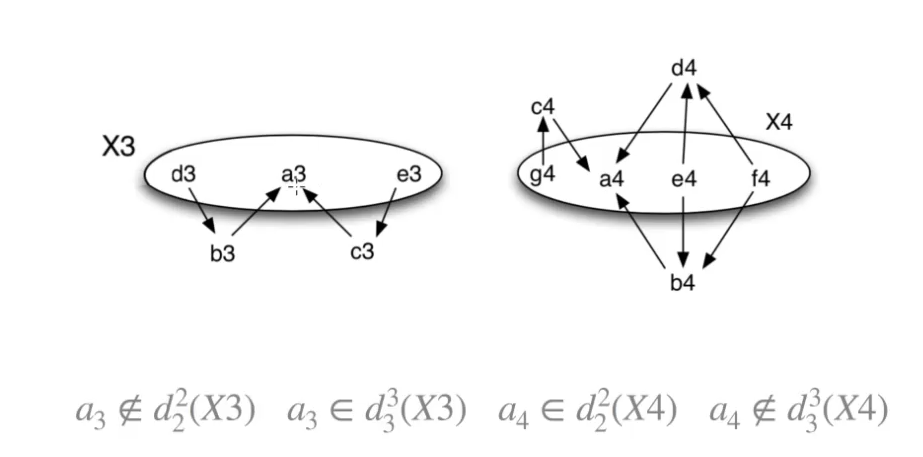
\includegraphics[width=13cm, keepaspectratio]{img/graded_sem_partial_order.png}
    \caption{Esempio graded defense partial order.}\label{fig:es_graded_defense_partial order}
\end{figure}

\begin{figure}[H]
    \centering
    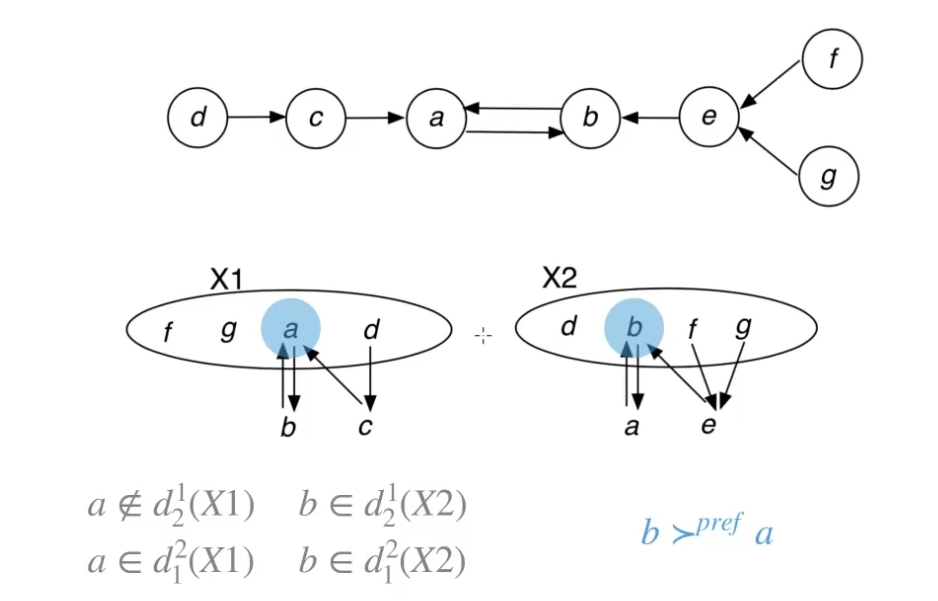
\includegraphics[width=13cm, keepaspectratio]{img/es_fin_graded_semantics.png}
    \caption{Applicazione di graded semantics a AF .}\label{fig:es_fin_graded_semantics}
\end{figure}
